\chapter{Deep Learning
and Transformer architecture}\label{chap:Model}
\section{Introduction to Deep Learning}\label{sec:DL}
Does our model magically learn to reconstruct input jets and distinguish between background and signal? No, it does not: it is nothing more than math formulas and in this chapter it is briefly discussed how it is done.\\
Deep Learning tries to replicate the behaviour of a human brain and, analogously, its basic unit is named "neuron" \cite{DLThesis}\cite{DLStanford}. From its dendrites it receives input values; they are processed and then summed in a weighted sum. After applying an activation function (described later), the signal is sent in output through the axon, towards the next dendrites. Neurons are organized in layers, constituting a network. The first one is defined \textit{input layer} and it receives original data as input; the last one is the \textit{output layer} and its output is the output of the model. Between them there are hidden layers, performing mathematical computations. A model with just one hidden layer is Perceptron. If the number of layers is large, the model is defined as Deep Network. 

\begin{figure}[h!]
    \centering
    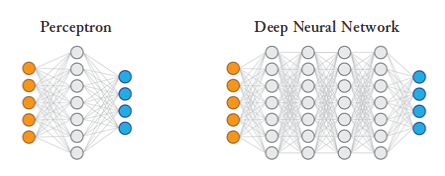
\includegraphics[width=3 in]{OLD/Images/Cap5/MLP&DNN.png}
    \caption{Comparison between a Perceptron and a Deep Network. Figure from Ref. \cite{DLThesis}}
    \label{fig:MLPDnn}
\end{figure}

\noindent The aim of a model training is to find the best function that connects input and output data. In order to achieve this goal, we reconstruct the function connecting a layer to the following, which is \cite{recoALGO}:
\begin{equation}\label{eq:weightsDL}
    O^L_i=\sigma \Big(\sum_jW^L_{ij}I^L_j+B_i^L\Big)
\end{equation}

\noindent where $I^L_i$ is the input vector, $O^L_i$ the input vector, $W^L_{ij}$ is the weight matrix (which has to be optimized during training), $B^L_i$ represents the bias vector for the layer $L$ and $\sigma$ is the activation function applied before signal leaves the neuron. When dealing with an hidden layer, we assume $I^L_i=O^{L-1}_j$. The activation function is a mathematical function setting a threshold to determine whether the neuron is active or not. In this thesis we used a GELU (Gaussian Error Linear Unit) activation \cite{GELU}. It is computed as follows:

\begin{equation}\label{eq:GELUcomplete}
    \sigma(x)=x\cdot\frac{1}{2}\Big[1+erf\Big(\frac{x}{\sqrt{2}}\Big)\Big]\simeq x\cdot\frac{1}{2}\Bigg[1+tanh\Big[\sqrt{\frac{2}{\pi}}(x+0.044715x^3)\Big]\Bigg]
\end{equation}

\noindent where the $erf$ function is defined as:

\begin{equation}
   erf (x)= \frac{2}{\sqrt{\pi}}\int_0^xe^{-t^2}dt
\end{equation}

\begin{figure}[h!]
    \centering
    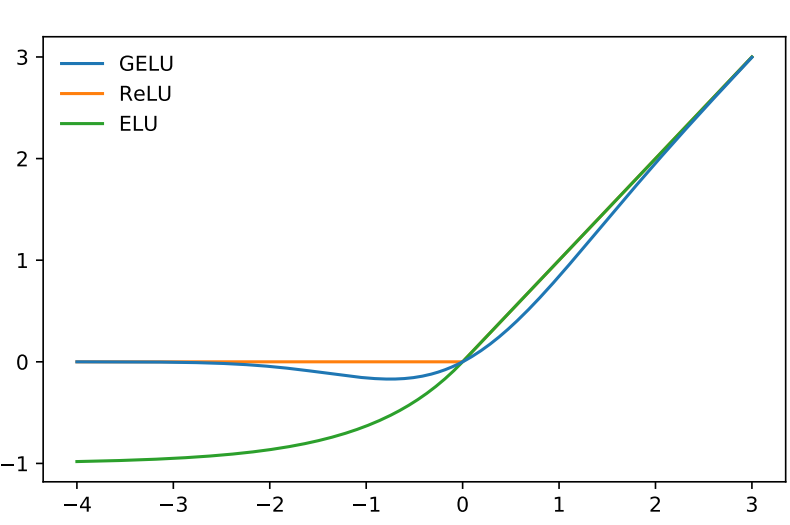
\includegraphics[width=3 in]{OLD/Images/Cap5/GELU.png}
    \caption[Caption for LOF]{Comparison between GELU, ReLU and ELU \footnotemark activation Figure from Ref. \cite{GELU}}
    \label{fig:GELU}
\end{figure}

\noindent As explained above, the model implementation is based on math and also the process of learning does. A loss function $\mathcal{L}$ is defined from the distance between the input and the output of the model. During the training phase we try to minimize this function adjusting weights of the model. A possible method to do so is the stochastic gradient descent (SGD). Defining \textbf{p}$\in \mathbb{R}^s$ as the vector containing weights and biases, SGD is computed \cite{DLThesis}:

\begin{equation}\label{eq:SGD}
    \mathbf{p} \rightarrow \mathbf{p}-\eta \Bigg(\frac{\partial \mathcal{L}}{\partial p_r}\Delta p_r\Bigg)_{x^{\{i\}}}
\end{equation}
\\
\noindent where $\eta$ is the learning rate, an hyperparameter that has to be optimized, computed as the ratio between the step size and the absolute value of the gradient. $\Delta p_r$ is a perturbation associated to the step. To calculate the gradient back-propagation is applied: weights are computed while forward feeding the model and then computed again when data passes backwards. Values are combined to present the best estimation of weights.

\footnotetext{ReLU = Rectified Linear Unit activation function; ELU = Exponential Linear Unit activation function}

%%%%%%%%
\section{Proposed model: Transformer architecture} \label{sec:Transformer}
In order to complete the Anomaly Detection task, we implemented a Transformer architecture, a model based on the Multi-Head Attention mechanism (MHA)\cite{attentionneed} \cite{GiaguTransf}. It is defined "Multi-Head" because it is implemented \textit{h} times simultaneously (\textit{h} stands for number of heads); it is "Attention" because it relies on the attention function, which maps a query and a set of key-value pairs to an output. The core aspect of this mechanism is that its weights are dynamic, meaning they change depending on the data that is passed as input. This feature allows the model to learn only the relevant parts of the dataset and, in our case, of the jets.\\
All just said is converted into concrete actions using the "Scaled Dot-Product Attention", which is a parallelism with the process of the retrieval in a database of a value \textit{v} based on a query \textit{q} and on a key \textit{k}. In our case, queries and keys, of a dimension $d_k$, are packed respectively into a matrix \textit{Q} and \textit{K}. Also values, of a dimension $d_v$, are presented as a matrix \textit{V}. The dot product of \textit{Q} with \textit{K} is computed and then we divide by $\sqrt{d_k}$. The output is still a matrix and it is computed as:
\begin{equation}\label{eq:Attention}
    Attention(Q,K,V)=\ \rm softmax\Bigg(\frac{\textit{Q} \textit{K}^T}{\sqrt{\textit{d}_k}}\Bigg)\textit{V}
\end{equation}

\begin{figure}[h!]
    \centering
    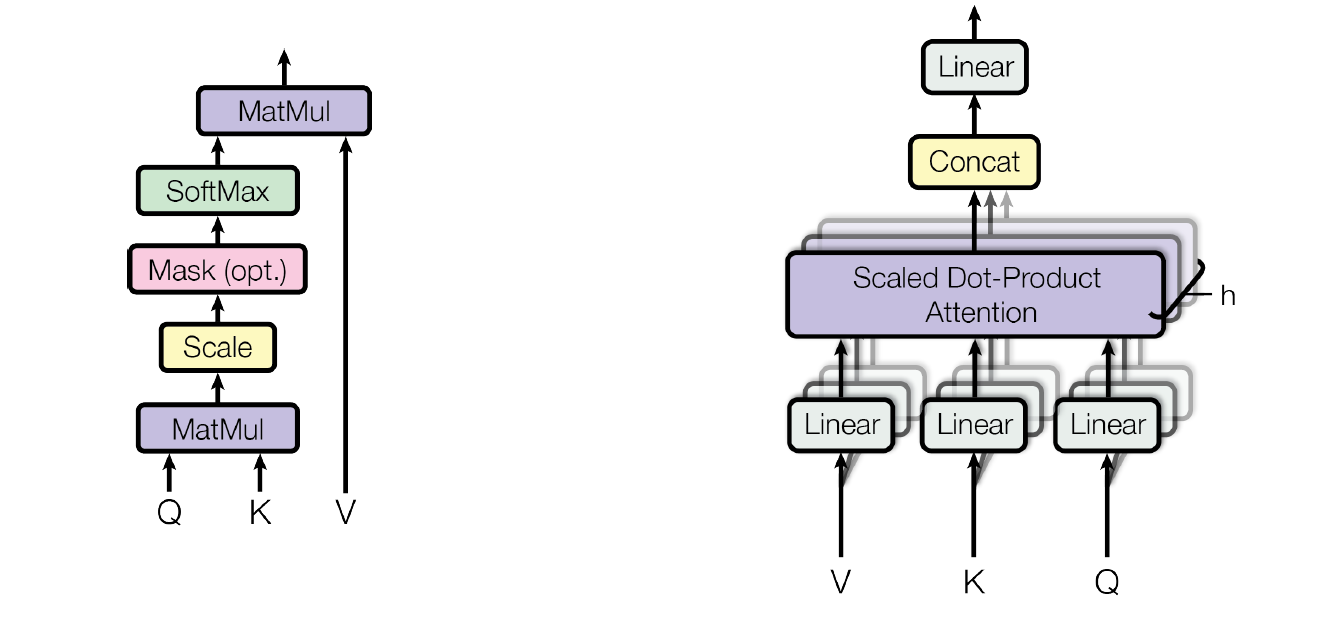
\includegraphics[width=3.5 in]{OLD/Images/Cap5/DOTandMHA.png}
    \caption{Scaled Dot-Product (left), MHA (right). Figure from Ref. \cite{attentionneed}}
    \label{fig:attentionBlock}
\end{figure}

\noindent Starting from the Scaled Dot-Product, we obtain the MHA computing in parallel multiple sets $i=1,…,h$ of keys, querys, and values, where $h$ is the number of heads applied. In fact, $Q, K, V$ are linearly projected in the respective dimension; then the attention mechanism is performed in parallel. Results are concatenated and projected, to give us MHA:
\begin{equation}\label{eq:MHA}
\begin{split}
    h_i(Q_i,K_i,V_i)=Attention(QW_i^Q,KW_i^K,VW_i^V)\\
    MHA(Q,K,V)=concat[h_1,h_2, ... , h_h]W^O\ \rm \ \rm \ \rm \ \rm \ \rm
\end{split}
\end{equation}

\noindent where the letter $W$ stands for the projections in the different dimensions: $W_i^Q\ \rm \in \mathbb{R}^{d_{model}\times d_k}$ , $W_i^K\ \rm \in \mathbb{R}^{d_{model}\times d_k}$ , $W_i^V\ \rm \in \mathbb{R}^{d_{model}\times d_v}$ and $W^O\ \rm \in \mathbb{R}^{hd_v\times d_{model}}$.\\
The number of heads $h$ is an hyperparameter that has to be optimized during the training phase, just as the learning rate.\\
MHA is the essential constituent of the Transformer architecture. This model has typically an encoder-decoder structure \ref{fig:Paper Transform}, meaning the input $x$ is mapped to a sequence of continuous representations $z$ by the encoder and then turned into output by the decoder. We are going to focus only on the encoder because it is the part of the model that we implement in this thesis.\\

\begin{figure}[h!]
    \centering
    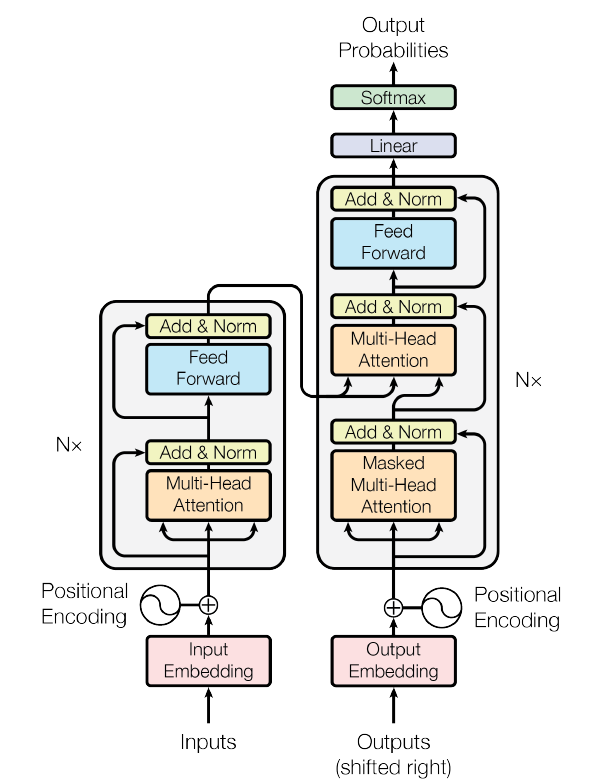
\includegraphics[width=2 in]{OLD/Images/Cap5/PaperTransf.png}
    \caption{Schematic of the implementation of the Transformer model in the paper \cite{attentionneed}}
    \label{fig:Paper Transform}
\end{figure}


\noindent The model is a stack of $L$ identical layers and each of them is composed by two sub-layers: MHA and a feed-forward network. The keys, values and queries to implement MHA in a layer are the output of the previous. The number of layers $L$ is an hyperparameter that has to be optimized. The output will be an embedding for each input data. 

%%%%%%%%%
\section*{Our Transformer implementation}\label{sec:myTransf}

\begin{figure}[h!]
    \centering
    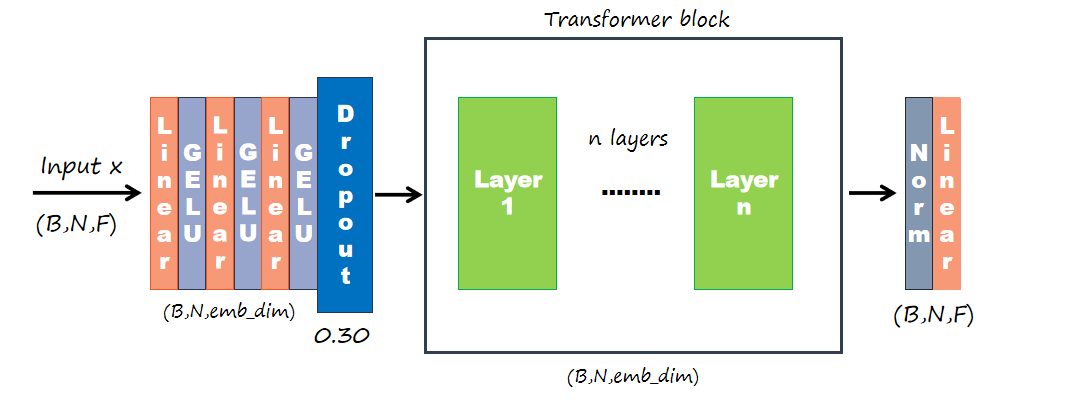
\includegraphics[width=4.5 in]{OLD/Images/Cap5/TransformerBlock.png}
    \caption{Schematic of our implementation of the Transformer model}
    \label{fig:MyTransformer}
\end{figure}


\noindent Based on what is said above and on what is presented in the original paper \cite{attentionneed}, an implementation of the Transformer architecture is developed. Right after that, to go back to the input dimension, a linear layer is applied. In figure \ref{fig:MyTransformer} a schematic of the implementation of the Transformer architecture is presented. Talking about dimensions, prior passing the training set of data to the model, the dataset is divided into batches of shape (512, 50, 3) which corresponds to the shape (B, N, F) in the schematic. Once our data is in, using a series of three linear layers followed by GELU activation (\ref{eq:GELUcomplete}), it is taken to the desired dimension (512, 50, 128). At this point, a dropout layer is applied. It is about dropping out the nodes of a few randomly selected neurons in order to avoid overfitting, as shown in figure \ref{fig:dropout}. The number of neurons involved depends on the probability associated to this process. In our case, a dropout of probability 0.30 is applied and then the vector is passed to $L$ layers of MHA (green rectangles in the picture). As said before, after this crucial phase, our vector is taken back to the input dimension applying a Layer Normalisation and a Linear Layer.

\begin{figure}[h!]
    \centering
    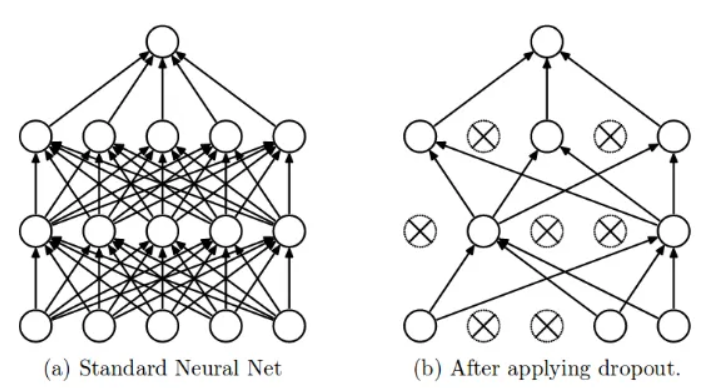
\includegraphics[width=2.5 in]{OLD/Images/Cap5/Dropout.png}
    \caption{Schematic of dropout}
    \label{fig:dropout}
\end{figure}

\begin{figure}[h!]
    \centering
    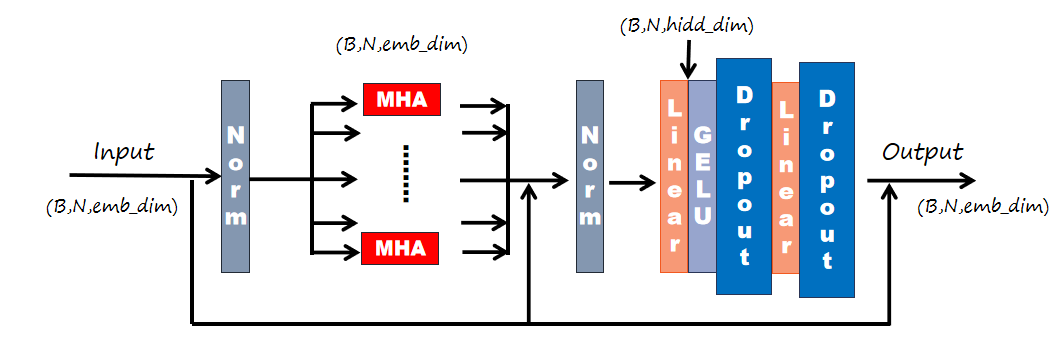
\includegraphics[width=4.5 in]{OLD/Images/Cap5/AttentionBlock.png}
    \caption{Schematic of our implementation of the MHA}
    \label{fig:MYattentionBlock}
\end{figure}

\noindent Finally, in figure \ref{fig:MYattentionBlock} our implementation of a layer of the model, containing the MHA is presented. It is basically quite similar to the original paper \cite{attentionneed}, where after a Layer Normalisation, MHA is applied \textit{h} times. Then the input is summed to this output. The difference between the paper and this work is that we propose that at the end of the layer, after a few more linear and dropout layers, we add the input vector to the current vector of data, instead of adding the output of the second normalisation. This difference was presented assuming that an additional information about the macro-structure of the jet would have helped the model in the discrimination phase. However, this difference has been proved to have a minor impact on the final result.